\subsubsection{Moving average filter} \label{sec:mavg_test}
Moving average filtret testes for at undersøge, hvorvidt de opstillede krav overholdes, samt undersøge om designet er korrekt implementeret. 
Filtret testes ved anvendelse af data fra pilotforsøget i \autoref{sec:pilotforsoeg}, da dette giver kontrollerede testforhold. 
MATLAB benyttes til at sende en given måling til mikrokontrolleren, hvorpå det digitale filter er implementeret. 
Mikrokontrolleren returnerer løbende den filtrerede værdi, der visualiseres i MATLAB. 
Ud fra dette ses om filtret udglatter signalet som forventet. 
Resultatet af denne test fremgår af \autoref{fig:mavg_test}. 

\begin{figure}[H]
	\centering
	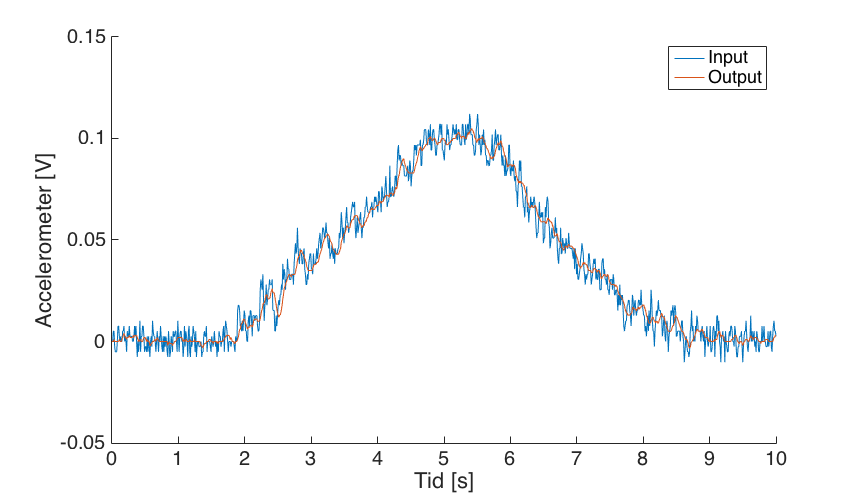
\includegraphics[width=1\textwidth]{figures/accelerometer_filter}
	\caption{Den blå graf illustrerer et samplet ufiltreret signal fra et accelerometer, og den røde graf illustrerer et opsamlet filtreret signal fra et accelerometer, visualiseret i MATLAB.}
	\label{fig:mavg_test}
\end{figure}

\noindent
%Da filteret kræver 10 samples for at retunere den første værdi testes det, hvorvidt dette stemmer overens med den forventede forsinkelse på $100~ms$. 
Der foretages yderligere en test med fremgangsmåde som den forrige. 
Hertil anvendes et square-wave signal genereret i MATLAB. 
Dette signal overføres til mikrokontrolleren, hvor filtret er implementeret, og det filtrerede data returneres. 
En visualisering af denne test ses på \autoref{fig:forsinkelse}.

\begin{figure}[H]
	\centering
	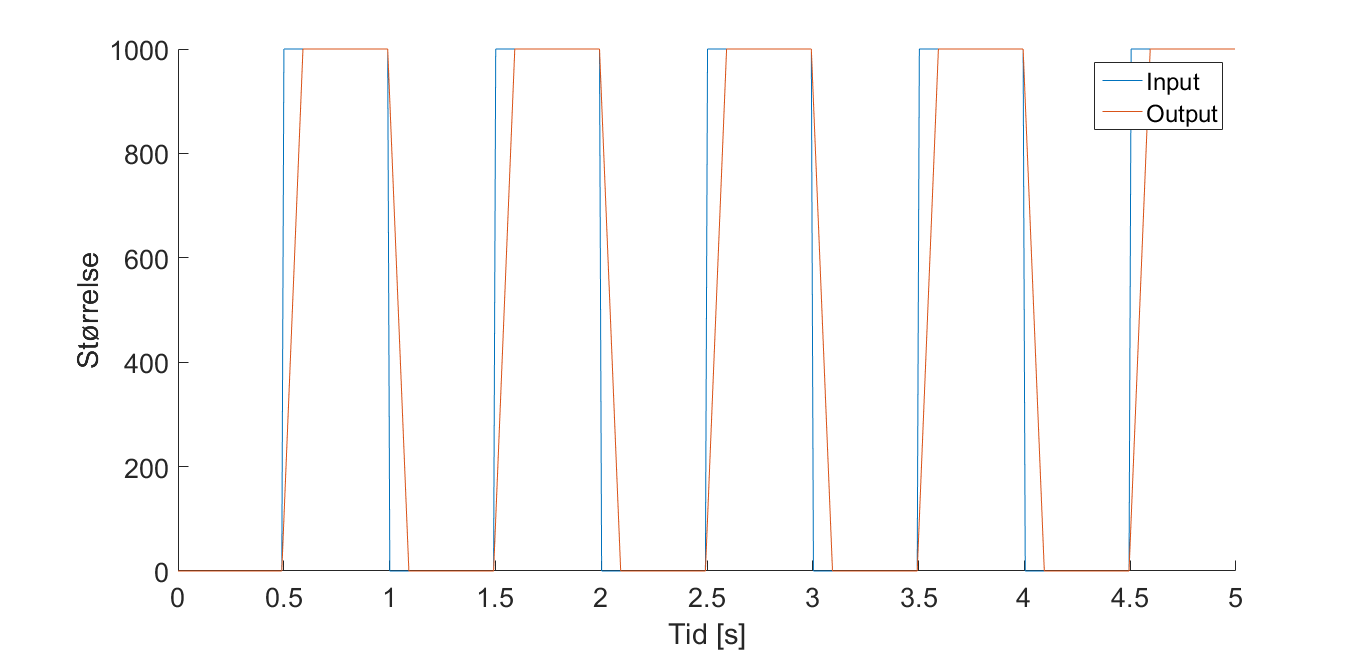
\includegraphics[width=1\textwidth]{figures/forsinkelse}
	\caption{Den blå graf illustrerer et genereret signal, og den røde graf illustrerer det samplede filtrerede signal.}
	\label{fig:forsinkelse}
\end{figure}

\noindent
Resultatet af denne test viser, at moving average filtret udglatter signalet. 
Hertil ses en stigning i det genererede signal før det filtrerede signal når den samme størrelse. 
Mellem dette går der $0,09~s$. 
Dette er passende til mængden af samples, som filtrets gennemsnit er udregnet ud fra, med en samplingsfrekvens på $100~Hz$. 
Dette er lavere end forventet, da der udfra $10~samples$ forventes at tage $0,1~s$, hvorfor filtret accepteres.  

Yderligere testes forsinkelsen, hvilken er udført som forklaret i \autoref{sec:lavpas_test}. 
Resultatet fra testen er en forsinkelse på $320~\mu s$ for data at passere filtret. 
Dette betragtes som ikke at være af signifikant betydning i forhold til det samlede system.    
Ud fra ovenstående resultater vurderes det, at filtret opfylder kravene i \autoref{sec:mavg_krav}. 

\vspace{3mm}
\textbf{Opsummering af krav:}
\begin{itemize}
\item[\text{\sffamily \checkmark}] Skal muliggøre en repræsentation af spændinger 
\item[\text{\sffamily \checkmark}] Skal have en filterlængde på $10$ samples
%\item[\text{\sffamily \checkmark}] Skal maksimal tage $100~ms$ for at opnå samme værdi som det oprindelige signal ved en konstant amplitude
\end{itemize}